\chapter{Komponenty}
\label{3-soucastky}

Při stavbě drona je potřeba rozmyslet účel drona, nosnost a délku letu. Od těchto myšlenek(potřeb) se odvíjí dílčí součástky a jejich parametry. Základní součátky jsou kostra, baterie, vrtule, bezkartáčové motory, regulátory otáček, IMU, komunikační zařízení a řídící jednotku.\\ Důležitým faktorem je i počet vrtulí/motorů.Podle počtu vrtulí dělíme drony na trikoptéry (3), quadrokopéry (4), hexakoptéry (6), a octokoptéry (8). Obecně platí čím více vrtulí dron má, tím více je stabilnější, dokáže létat i při selhání z jednoho motorů (hexakoptéra a octokoptéra). Zároveň stavba drona s vyšší počtem vrtulí je dražší a náročnější.

V této diplomové práci je popisována stavba hexakoptéry, jejíž kostra a motory byly použity z nefukčního drona of firmy Microkopter z laboratoře fotogrametrie.

\section{Kostra} 
Kostra by měla být lehká a pevná, nejčastěji se používá karbon a hliník pro stavbu drona s vyšší nosností a plast pro ostatní drony. Kostra se skládá z centra, ramen, stojánku a držáků pro motory.
Jak už bylo zmíněno, byla použita kostra od firmy Microkopter. Stojánek je vyroben z karbonu, centrum z plastu a ramena a držáky motorů z hliníku.

\section{Baterie} 
Výběrovým kritériem pro baterie jsou kapacita, výstupní napětí, maximální vybíjecí proud.
Nejpoužívanějšími bateriemi pro stavbu drona jsou LiPo baterie, které nejsou příliž těžké, nemají paměťový efekt, mají dlouhou životnost při správném zacházení a vysoký vybíjecí proud.\\
Kapacitu a výstupní napětí ovlivňuje množství článků baterie. 
Jeden článek má hodnotu nominálního napětí 3.7V, při plném nabití článku 4.2V. Maximální vybíjecí proud je dán hodnotou C. Pokud C je rovno 25 a kapacita baterie je 6750 mA, můžeme z baterie odebírat proud o velikosti cca 168 Ampérů. 6.75*25 = 168.75A
Maximální odběr by neměl přesáhnout, protože potom se poškozuje baterie.

\subsection{Parametry použité baterie} 
%https://www.peckamodel.cz/ta-25c-6750-4s1p-gens-ace-lipo-tattu-serie-4s-6750-mah-25c\\
Počet článků: 4 (4S)\\
Napětí: 14.8V\\
Kapacita baterie: 6750mA\\
Maximální proudové zatížení: 25C (168.75A)\\
Maximální vybíjecí proud: 50C (337.5A)\\
Hmotnost: 605 g\\

\subsection{Rady pro zacházení s LiPo bateriemi} 
Nabíjet baterie proudem s 1C tedy 6750mA dobíjet 6.75A proudem.\\
Nepřebíjet baterie nad hodnotu napětí 4.2V na článek.\\
Nepodbíjet baterie pod napětí 2.7V, hrozí poškození.\\
Při delším skladování vybít na hodnotu napětí 3.3V na článek.\\
Pro podrobnější instrukce je potřeba si přečíst příbalový leták.\\

\section{Distribuční deska} 
Distribuční deska PCB neboli napájecí deska slouží k zapojení všech  komponent na baterii. Jednotlivá napájená místa jsou zapojena paralelně, aby při zkratu jednoho ze zařízení, ostatní zařízení fungovala. K desce lze připojit i zařízení s jiným vstupním napětím než je napětí baterie (5V, 12V).

\subsection{Parametry distribuční desky}
Matek PDB-XT60\\
Množství LiPo článků: 3S-4S\\
Vstup VCC, GND\\
Výstup, 6x + a -, 12V, 5V, 2x -\\
%https://www.rotorama.cz/prislusenstvi/matek-pdb-s-5v-12v

\begin{figure}[h]
	\centering
	\includegraphics[width=3cm]{pictures/pdb.jpg}
	\caption{Distribuční deska - Matek PDB-XT60}
\end{figure}

\section{Vrtule} 
Vrtule generují tah dronu.Při stavbě drona jsou potřeba dva typy vrtulí se směrem hodinových ručiček a proti. Dva typy vrtulí jsou potřeba pro rotaci drona kolem svislé osy. Další parametry vrtulí je jejich průměr a rozteč, nejčastěji uvedená v palcích. Materiál použit na výrobů vrtulí je plast nebo karbon. Doporučuji při stavbě drona a jeho testování použít plastové vrtule, jsou cenově méně náročné.

\subsection{Parametry použitých vrtulí} 
Materiál: plast
Průměr: 12 palců\\
Rozteč: 3.8 palce\\

\section{Bezkartáčové motory} 
%https://www.youtube.com/watch?v=bCEiOnuODac
%https://www.mikrocontroller.com/index.php?main_page=product_info&cPath=73&products_id=887&zenid=e5f2c8d548f2a39747a4ed06d306a37f
BLDC motory mají výhodu především v dlouhé životnosti a plynulém kroku. BLDC motor se skládá z rotoru a statoru. Rotor je permanentní magnet, stator je prstenec uspořádaných cívek. Postupným pouštění proudu do cívek (vytvařením magnetického pole) se rotor začne pohybovat. Cívky jsou rozdělené do skupiny A, B, C, což jsou i vstupní piny motorů.  Nedílnou součástí motorů je regulátor otáček ESC, který řídí vstupní proud přes piny A, B a C a tím ovlivnujě rychlost motoru.
Pin B je prosřední. Napájením pinů A a C určíme směr otáčení motoru, možnost otáčení lze i změnit v nastavení regulátoru otáček.
Výběr motorů je závislý na parametrech baterie a parametrech regulátoru otáček.

\subsection{Parametry použitých motorů} 
Firma: Microkkopter\\
Množství LiPo článků: 4S-6S\\
Provozní napětí: 25A\\
Maximální provozní napětí 30A\\
Rychlost bez zatížení: 500 rpm/V\\
Nosnost: 2200g\\
Váha: 121g\\

\section{Regulátory otáček} 
Regulátory otáček (ESC) jsou nedílnou součástí BLDC motorů. Regulátor je řídící jednotka motoru, která zajistí jeho plynulý chod.

Vstupní napětí zaleží dle typu regulátoru
Regulátory se ovládájí přes PWM signál s frekvencí 50Hz. Přes PWM signál se posílá údaj throttle, které uvádá výkon motoru. Každý regulátor má jinak definovanou minimální a maximální hodnotu throttle, proto je potřeba regulátory kalibrovat.

\subsection{Parametry použitých regulátorů otáček}
HGLRC BS30A\\
Vnitřní software: BLHeliSuite\\
Vstup: VCC (7.4V - 18.5V) ,GND, -, S\\
Výstup: A, B, C\\
Maximální proud: 30A / 40A max\\
Množství LiPo článků: 2S-5S\\
Použitá knihovna: Servo\\

\begin{figure}[h]
	\centering
	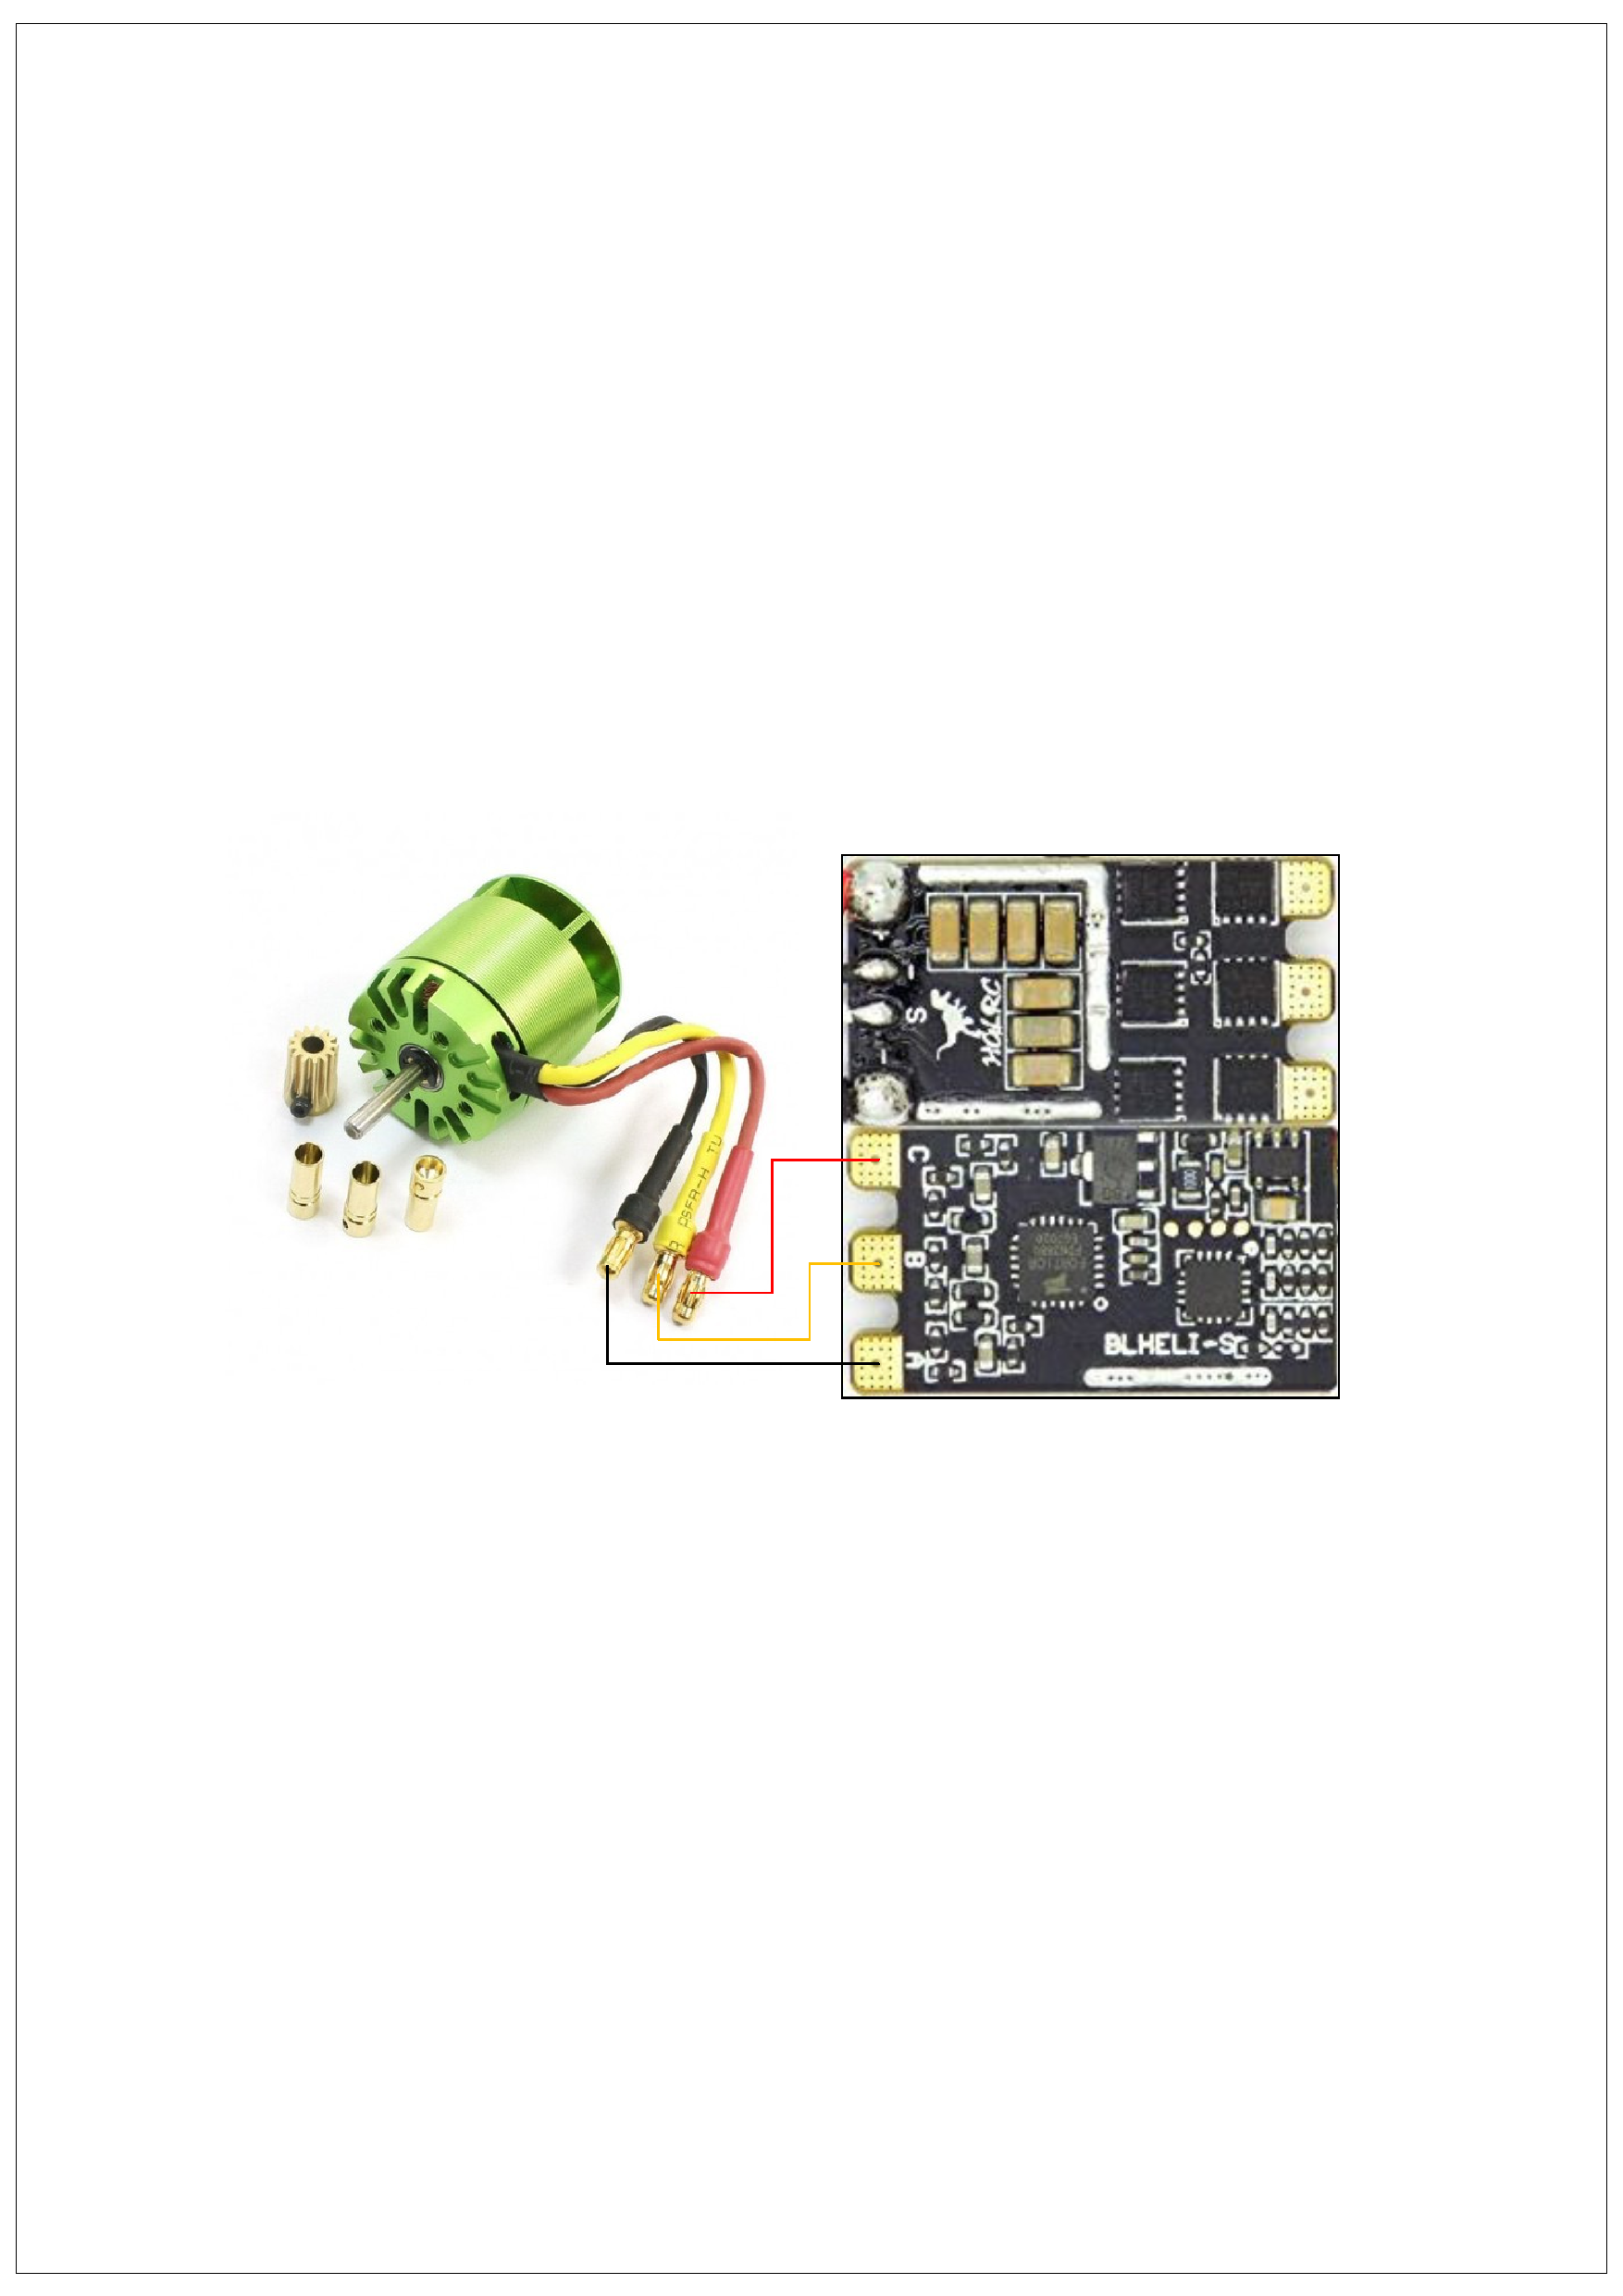
\includegraphics[width=4cm]{pictures/esc.jpg}
	\caption{Regulátor otáček - HGLRC BS30A}
\end{figure}

\begin{figure}[h]
	\centering
	\includegraphics[width=8cm]{pictures/motor.pdf}
	\caption{Schéma zapojení motoru a regulátoru}
\end{figure}

\section{IMU}
IMU je zařízení, které měří úhlové rychlosti, zrychlení a sil magnetické pole ve třech osách. Skládá se z gyroskopu, akcerelometru  magnetometru. !9 stupnu volnosti!

\subsection{Akcelerometr}
Akcelerometr slouží k určování zrychlení. Elektronický akcelerometr měří zrychlení na základě  změny elektrické kapacity mezi pevnou částí a pohyblivou částí akcelerometru. 

\subsection{Gyroskop}
Gyroskop slouží k úhlové rychlosti. Elektronický gyroskop měří úhlové rychlosti také na základě změny elektrocké kapacity, ale změnu měří ve dvou směrech na sobě kolmých. Z těchto dvou změn se vypočte úhel stočení.

\subsection{Magnetometr}
Magnetometr slouží k určování sil magnetického pole Země. Elektronický magnetometr využívá Hallův efekt, kdy vodivý plát je zasazen do elektronického obvodu. Při vlivu magnetického pole se na stranách plánu přidruží elektrony a protony. Měřené napětí na stranách plátu je úměrné k síle magnetického pole.

\subsection{Parametry použité IMU jednotky}
Arduino modul MPU9250\\
Obsahuje: akcelerometr, gyroskop, magnetometr\\
Komunikace: I2C, SPI\\
Vstup: VCC (5V), GND\\
Výstup: SDA, SCL (I2C)\\
Použitá knihovna: MPU9250\\
%https://github.com/bolderflight/MPU9250
Souřadný systém akcelerometru a gyroskopu je shodný, magnetometr má opačnou osu z a prohozené osy x a y.
%https://www.invensense.com/wp-content/uploads/2015/02/PS-MPU-9250A-01-v1.1.pdf

\begin{figure}[h]
	\centering
	\includegraphics[width=3cm]{pictures/imu.jpg}
	\caption{IMU - MPU9250}
\end{figure}
 
\section{Komunikační zařízení} 
Pro bezdrátové ovládání drona je použit radiový modul a bluetooth

\subsection{Radio} 
Radiový modul je použáván pro zvětšení dosahu ovládání drona. Pro stavbu byl použit bezdrátový modul XBee od firmi Digi. Modul plní funkce koncového zařízení, routeru nebo koordinátoru. Komunikace s XBee probíhá přes UART. Modul lze použít i pro čtení analogových a digitálních signálů různých senzorů.

\subsection{Parametry použitého Radiového zařízení}
XBEE PRO SS\\
Provozní napětí: 3.3V\\
Provozní frekvence: 2.4GHz\\
Komunikační protokol: ZB ZigBee\\
Dosah:12 km\\

%https://www.proto-pic.co.uk/user/products/large/08665-03-L__99538__33841.jpg
\begin{figure}[h]
	\centering
	\includegraphics[width=5cm]{pictures/xbee.jpg}
	\caption{XBee}
\end{figure}

\subsection{Bluetooth} 
Pro bezdrátovou komukaci s telefonem byl použit Arduino Bluetooth modul. Při zapojení je potřeba připojit RX pin modulu na TX pin Arduina a TX pin modulu na RX pin Arduina, aby komunikace fungovala.

\subsection{Parametry použitého Bluetooth zařízení}
HC-05\\
Bluetooth verze: 2.0\\
Výchozí rychlost komunikace: 9600 baudů\\
Vstup: VCC (5V), GND, RX, EN\\
Výstup: TX, STATE\\
Použitá knihovna: SoftwareSerial\\

\begin{figure}[h]
	\centering
	\includegraphics[width=5cm]{pictures/blue.jpg}
	\caption{Bluetooth - HC-05}
\end{figure}

\section{Řídící jednotka} 
Pro ovládání všech kompoment byla použita platforma Arduino.

\subsection{Arduino} 
Arduino je otevřená vývojová platforma, která využívá mikroprocesory od firmy Atmel. Programovat Arduino lze přes jazyk C nebo C++. Pro začínají uživatele byla vytvořena knihovna Wiring, která je velmi rozšířená. Knihovna je integrovaná do vývojového prostředí Arduino IDE. Na trhu existuje spousta typů desek např. Uno, Nano, Mega, Due. \\
Arduino lze napájet přes 12V konektor, USB nebo VIN, vstupní napětí má být v rozsahu 5V - 12V. Vstupy Arduina jsou Buď analogové nebo digitální. Rozsah analogových vstupů je 0-1023. Digitální vstupy mají hodnotu LOW nebo HIGH, přenos dat probíhá přes PWM, I2C nebo UART komunikaci. Pro každou komunikaci jsou definovány určité digitálních pinů. I2C komunikace je továrně nastavena na analogové piny dle typu desky.\\
Jelikož Arduino je open-source projekt, vzniká tak spousta klonů a nadstaveb. U projektu autonomního letadla byl použit levnější klon.\\


\begin{figure}
	\centering
	\includegraphics[width=5cm]{pictures/uno.jpg}
	\includegraphics[width=5cm]{pictures/nano.jpg}
	\caption{Arduino UNO a Nano}
\end{figure}

\section{GNSS}
Informace o GNSS aparatuře jsou k dispozici v diplomové práci Štěpána Hodíka.

\section{Výškoměr}
Pro funkci výškoměru byla požita dvě zařízení: barometr a gps.

\subsection{Barometr}
Barometrem měříme tlak a z tlaku lze vypočítat nadmořská výška.

\subsection{Použitý barometr}
BMP280\\
Vstup: VCC (3.3V), GND,\\
Výstup: SDA, SCL, SDO, CSB\\
Měřící rozsah teploty:-40 až +85 stupňů\\
Měřící rozsah tlaku:300 až 1100 hPa\\
Přesnost měření teploty: +- 1 stupeň\\
Přesnost měření tlaku:  +- 100 Pa\\
Použitá knihovna: Adafruit BMP280\\
%https://github.com/adafruit/Adafruit_BMP280_Library

\begin{figure}[h]
	\centering
	\includegraphics[width=2cm]{pictures/baro.jpg}
	\caption{Barometr - BMP280}
\end{figure}

\section{Senzor překážek/vzdáleností}
Pro automatizaci je důležíté opatřit drona senzory měřící vzdálenosti pro předcházení srážek s objekty. Senzory byly připevněny na ramena vrtulí pro měření vzdáleností ve vodorovné rovině drona a pro měření ve svislém směru pro přistávání a detekce objektů pod dronem.

\subsection{Použíty laserový modul}
laserový modul Vl53l0x\\
Vstup: VCC (5V), GND, XSHUT, GPIO1\\
Výstup: SDA, SCL (I2C)\\
vlnová délka: 940 nm\\
měřící rozsah: 0 - 1200 mm\\
přesnost: 3 procenta měřené délky\\
Použitá knihovna: VL53L0X\\
%https://github.com/pololu/vl53l0x-arduino

\begin{figure}[h]
	\centering
	\includegraphics[width=2cm]{pictures/laser.jpg}
	\caption{Laserový modul - Vl53l0x}
\end{figure}

Při používání pouze jednoho modulu stačí propojit pouze 4 pin VIN, GND, SCL, SDA. Pro více modulů je potřeba zapojit pin XSHUT na některý z digitálních pinů. Pin XSHUT k přepnutí modulu do stan-by režimu, pro definování adresy, přes I2C komunikaci, na používaném modulu.

\section{Kamera}
Pro obrazový věm letu drona byl nainstalován systém FPV.  FPV se skládá z kamery, vysílače, přijímače a obrazového media. Kamera předává obrazová data radiovému vysílači, který je na určité frekvenci posílá přijímači. Přijímač signál dekoduje a zobrazí na mediu.

\subsection{Použítá kamera}
Eachine TX02\\
Vstup: VCC (5V), GND\\
Výstup: radiový signál s frekvencí 5.8GHz\\
FOV: 120 stupnu\\
Rozlišení: 600TVL\\
Použitá Android aplikace: FPViewer\\